\documentclass[tikz, border=10pt]{standalone}
\usepackage{tikz}
\usepackage{amsmath}
\usepackage{xcolor}
\usetikzlibrary{arrows.meta, shapes.geometric, positioning, fit,
                backgrounds, calc, decorations.pathreplacing}

\definecolor{navybg}{HTML}{0d1b2a}
\definecolor{stageA}{HTML}{00bcd4}   % Source Synthesis
\definecolor{stageB}{HTML}{26a69a}   % Spatialization
\definecolor{stageC}{HTML}{66bb6a}   % Fractional Delay
\definecolor{stageD}{HTML}{ffa726}   % Noise Mixing
\definecolor{stageE}{HTML}{ef5350}   % Dataset Assembly
\definecolor{outputCol}{HTML}{b0bec5}

\tikzset{
  stagenode/.style 2 args={
    draw=#1, fill=#1!18, very thick,
    rectangle, rounded corners=6pt,
    minimum width=3.6cm, minimum height=2.8cm,
    text=#1, font=\sffamily\footnotesize, align=center
  },
  shapearrow/.style={->, very thick, #1}
}

\begin{document}
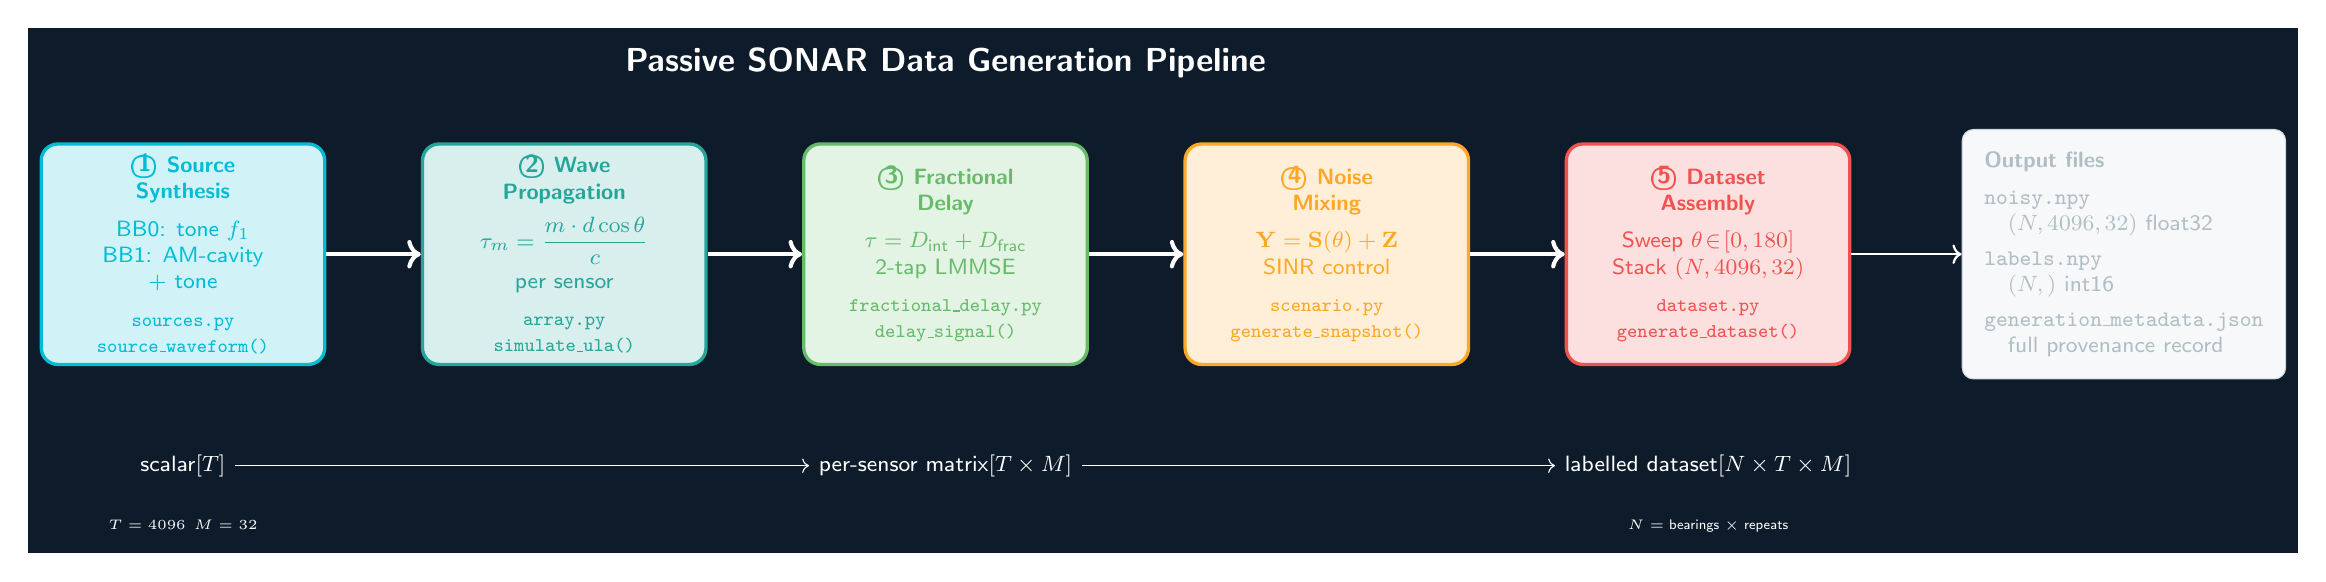
\begin{tikzpicture}[
    font=\sffamily\small,
    background rectangle/.style={fill=navybg},
    show background rectangle,
    every node/.style={text=white}
]

%% ── Stage boxes ──────────────────────────────────────────────────────────
\node[stagenode={stageA}{}, text=stageA] (st1) at (0, 0) {
    \textbf{\textcircled{\small 1} Source}\\
    \textbf{Synthesis}\\[4pt]
    BB0: tone $f_1$\\
    BB1: AM-cavity\\
    $+$ tone\\[4pt]
    \texttt{\scriptsize sources.py}\\
    \texttt{\scriptsize source\_waveform()}
};

\node[stagenode={stageB}{}, text=stageB, right=1.2cm of st1] (st2) {
    \textbf{\textcircled{\small 2} Wave}\\
    \textbf{Propagation}\\[4pt]
    $\tau_m = \dfrac{m \cdot d\cos\theta}{c}$\\[4pt]
    per sensor\\[4pt]
    \texttt{\scriptsize array.py}\\
    \texttt{\scriptsize simulate\_ula()}
};

\node[stagenode={stageC}{}, text=stageC, right=1.2cm of st2] (st3) {
    \textbf{\textcircled{\small 3} Fractional}\\
    \textbf{Delay}\\[4pt]
    $\tau = D_{\text{int}} + D_{\text{frac}}$\\
    2-tap LMMSE\\[4pt]
    \texttt{\scriptsize fractional\_delay.py}\\
    \texttt{\scriptsize delay\_signal()}
};

\node[stagenode={stageD}{}, text=stageD, right=1.2cm of st3] (st4) {
    \textbf{\textcircled{\small 4} Noise}\\
    \textbf{Mixing}\\[4pt]
    $\mathbf{Y} = \mathbf{S}(\theta) + \mathbf{Z}$\\
    SINR control\\[4pt]
    \texttt{\scriptsize scenario.py}\\
    \texttt{\scriptsize generate\_snapshot()}
};

\node[stagenode={stageE}{}, text=stageE, right=1.2cm of st4] (st5) {
    \textbf{\textcircled{\small 5} Dataset}\\
    \textbf{Assembly}\\[4pt]
    Sweep $\theta\!\in\![0°,180°]$\\
    Stack $(N,4096,32)$\\[4pt]
    \texttt{\scriptsize dataset.py}\\
    \texttt{\scriptsize generate\_dataset()}
};

%% ── Connecting arrows ────────────────────────────────────────────────────
\foreach \from/\to in {st1/st2, st2/st3, st3/st4, st4/st5}{
    \draw[shapearrow={white}, line width=1.5pt]
        (\from.east) -- (\to.west);
}

%% ── Data shape transformation row (below stages) ─────────────────────────
\node[white!70, font=\sffamily\footnotesize, below=1.0cm of st1]
    (sh1) {scalar\\$[T]$};
\node[white!70, font=\sffamily\footnotesize, below=1.0cm of st3]
    (sh2) {per-sensor matrix\\$[T \times M]$};
\node[white!70, font=\sffamily\footnotesize, below=1.0cm of st5]
    (sh3) {labelled dataset\\$[N \times T \times M]$};

\draw[->, white!50, thin] (sh1.east) -- (sh2.west);
\draw[->, white!50, thin] (sh2.east) -- (sh3.west);

\node[white!40, font=\sffamily\tiny, below=0.3cm of sh1]
    {$T = 4096$\;\;$M = 32$};
\node[white!40, font=\sffamily\tiny, below=0.3cm of sh3]
    {$N = $ bearings $\times$ repeats};

%% ── Output files (right of stage 5) ─────────────────────────────────────
\node[draw=outputCol!60, fill=outputCol!10, rounded corners=4pt,
      text=outputCol, font=\sffamily\footnotesize, align=left,
      inner sep=8pt, right=1.4cm of st5] (outbox) {
    \textbf{Output files}\\[4pt]
    \texttt{noisy.npy}\\
    \quad$(N, 4096, 32)$ float32\\[3pt]
    \texttt{labels.npy}\\
    \quad$(N,)$ int16\\[3pt]
    \texttt{generation\_metadata.json}\\
    \quad full provenance record
};
\draw[->, white!70, thick] (st5.east) -- (outbox.west);

%% ── Top label ────────────────────────────────────────────────────────────
\node[white, font=\sffamily\large\bfseries]
    at ($(st1.north)!0.5!(st5.north) + (0, 1.0)$)
    {Passive SONAR Data Generation Pipeline};

\end{tikzpicture}
\end{document}
